\begin{figure}[t!]
\centering
\begin{subfigure}{.5\textwidth}
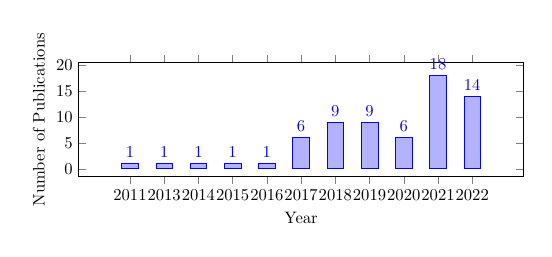
\begin{tikzpicture}[scale=0.6]
\begin{axis}  
[  
    ybar,  
    enlargelimits=0.15,  
    width=11cm,
    height=4cm,
    ylabel={Number of Publications}, 
    xlabel={Year},  
    symbolic x coords={2011, 2013, 2014,2015,2016, 2017, 2018, 2019, 2020, 2021, 2022}, 
    xtick=data,  
     nodes near coords,
    nodes near coords align={vertical},  
    ]  
\addplot coordinates {
(2022, 14)
(2021, 18)
(2020, 6)
(2019,9)
(2018,    9)
(2017,   6)
(2016,   1)
(2015,    1)
(2014,   1)
(2013,   1)
(2011,1)
};  
\end{axis}  
\end{tikzpicture}
\label{fig:pub_trends1}
\end{subfigure}%
\begin{subfigure}{.5\textwidth}
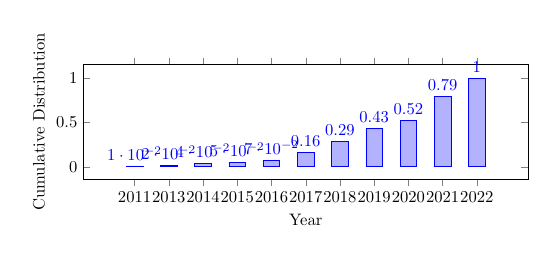
\begin{tikzpicture}[scale=0.6]
\begin{axis}  
[  
    ybar,  
    enlargelimits=0.15,  
    width=11cm,
     height=4cm,
    ylabel={Cumulative Distribution}, 
    xlabel={Year},  
    symbolic x coords={2011, 2013, 2014, 2015,2016, 2017, 2018, 2019, 2020, 2021, 2022}, 
    xtick=data,  
     nodes near coords,
    nodes near coords align={vertical},  
    ]  
\addplot coordinates {
(2011,0.01)
(2013,0.02)
(2014,0.04)
(2015,0.05)
(2016,0.07)
(2017,0.16)
(2018,0.29)
(2019,0.43)
(2020,0.52)
(2021,0.79)
(2022,1)
};  
\end{axis}  
\end{tikzpicture}
\label{fig:pub_trends2}
\end{subfigure}%
\newline
\caption{Publication trend of vulnerability detection studies.}
\label{fig:pub_trends}
\end{figure}
% \song{value of 2021 should not be 1} \nima{working on this}}
